\chapter{Theoretical Framework}
\label{theoretical-framework}

\section{Fundamentals of Language Learning}

\subsection{Language Acquisition Theories}

The field of \gls{sla} has evolved significantly in recent decades, moving from behaviorist approaches to more cognitive and sociocultural perspectives, and more recently, towards the integration of \gls{ia} technologies and adaptive systems that promise to revolutionize the way languages are learned.

Among the most influential theories in second language acquisition, the work of \cite{krashen1982principles} stands out, who developed the Monitor Model. This model includes five fundamental hypotheses, the most relevant being the comprehensible input hypothesis, which establishes that acquisition occurs when students receive input slightly above their current level of competence.

For his part, \cite{ellis1994study} proposes a more integrative theoretical framework, emphasizing the interaction between cognitive and environmental factors in language learning. His work highlights the importance of considering both internal mental processes and contextual variables that influence language acquisition, providing a solid theoretical foundation for understanding how students process and acquire a second language.

\subsection{Factors Influencing Second Language Learning}

\cite{ellis1994study} identifies various factors that affect language learning, which can be classified as internal and external.

Internal factors include the learner's age, linguistic aptitude, motivation and attitude, cognitive styles and learning strategies, as well as personality traits. Age influences brain plasticity and natural language acquisition capacity, while linguistic aptitude varies among individuals and can predict success in learning. Motivation can be intrinsic or extrinsic, and cognitive styles and learning strategies determine how information is processed and retained. Personality traits, such as extroversion, affect the willingness to participate in communicative interactions.

On the other hand, external factors include social and cultural context, exposure to the target language, and the quality and quantity of input. The learning environment and sociocultural context significantly influence attitudes toward the target language and its speakers, largely determining learning success.

Frequent and varied exposure to the language is fundamental for developing linguistic competence, and the input must be comprehensible yet challenging, following the i+1 principle of \cite{krashen1982principles}. This principle suggests that optimal learning occurs when the student is exposed to content slightly above their current level of competence.

Additionally, factors such as socioeconomic status, access to educational and technological resources, and linguistic policies of the environment also significantly influence the learning process. The availability of authentic materials and modern technological tools can considerably enrich the learning experience and facilitate exposure to the target language in meaningful contexts.

\subsection{Teaching Methodologies}
The evolution of teaching methodologies reflects our changing understanding of the language learning process:

\subsection{Traditional Methods}

The Grammar-Translation Method, predominant during the 19th and early 20th centuries \cite{richards2000approaches}, focuses on detailed analysis of grammatical rules and the translation of texts. This method emphasizes grammatical accuracy and reading comprehension, although it has been criticized for its limited attention to oral communication skills.

The Direct Method, introduced by \cite{gouin1892art}, emerged as a response to the limitations of the previous method, promoting total immersion in the target language and avoiding the use of the native language. This approach emphasizes the importance of oral communication and the direct association between language and meaning, without resorting to translation.

The Audiolingual Method, developed during World War II and founded by \cite{fries1945teaching}, is based on behaviorist principles and emphasizes the formation of linguistic habits through repetition and reinforcement. This method uses pattern drills and memorized dialogues to develop automaticity in language use.

\subsection{Modern Approaches}

The Communicative Language Teaching Approach \cite{hymes1972communicative} marked a revolutionary change in language teaching by emphasizing communicative competence over mere grammatical accuracy. This approach fundamentally transformed the way languages are taught, prioritizing meaningful interactions and language use in real contexts.

Task-Based Learning \cite{nunan1989designing} represents another fundamental pillar, organizing learning around authentic communicative activities. Its effectiveness lies in promoting natural language learning while students focus on completing practical and meaningful tasks.

Content and Language Integrated Learning \cite{coyle2010clil} has proven particularly effective by integrating academic content learning with language acquisition. This dual approach not only improves learning efficiency but also significantly increases student motivation by providing a relevant context and clear purpose for language use.

\subsection{Challenges in Learning Personalization}

Learning personalization represents one of the greatest challenges in language teaching. As \cite{ellis1994study} points out, a first fundamental challenge is the precise identification of the student's level, which requires comprehensive assessments that consider not only grammatical and lexical knowledge but also communicative skills in various contexts.

Adapting content to different learning styles constitutes another significant challenge, as it involves developing materials and activities that meet the individual preferences and needs of students, considering their different ways of processing and retaining linguistic information. \cite{krashen1982principles} emphasizes the importance of providing comprehensible input adapted to each student's individual level.

Maintaining motivation requires a delicate balance between challenge and support, needing strategies that maintain the student's interest and commitment over time. This is closely related to tracking individual progress, which must be continuous and detailed to allow timely adjustments in the learning process.

The scalability of personalized attention presents a particular challenge in educational contexts with limited resources, where it is necessary to find efficient ways to provide individualized feedback and personalized support to a large number of students simultaneously. This specific challenge motivates the implementation of \gls{ia}-based systems, particularly those using \gls{rl} and \gls{transformers} architectures, which can provide personalized attention at scale while maintaining instruction quality.

\subsection{Progress Evaluation}

Effective progress evaluation in language learning requires a multidimensional and systematic approach. \cite{ellis1994study} emphasizes that communicative competence, which encompasses both linguistic knowledge and the ability to use it appropriately in social contexts, must be evaluated through tasks that reflect authentic communicative situations.

Grammatical accuracy, although it should not be the sole focus of evaluation, needs to be monitored to ensure that students develop an adequate mastery of fundamental linguistic structures. This evaluation must be balanced with the measurement of fluency, which reflects the student's ability to communicate effectively and naturally in real-time.

\cite{krashen1982principles} maintains that listening and reading comprehension require specific evaluations that consider different types of texts and discourses, as well as various communicative purposes. These evaluations must measure both global comprehension and the ability to identify specific details.

Progress evaluation and contextual feedback are crucial elements that can significantly benefit from the integration of advanced technologies. Systems based on \gls{llm} and \gls{tts} and \gls{stt} technologies can provide more precise and detailed evaluations of the student's linguistic skills. These systems can analyze error patterns, identify areas for improvement, and provide personalized feedback in real-time, overcoming the limitations of traditional evaluation methods.




\section{Artificial Intelligence in Education}

The integration of \gls{ia} in the educational field has fundamentally transformed the way the teaching-learning process is conceived and implemented. This section explores the evolution and current state of intelligent educational systems, with special emphasis on their application in language teaching.

\subsection{Evolution of Adaptive Learning Systems}
Adaptive learning systems have evolved significantly since the first \gls{its} of the 1970s. VanLehn \cite{vanlehn2011relative} notes that this evolution has gone through three main generations: rule-based systems, domain knowledge-based systems, and modern adaptive systems that use machine learning and \gls{ia} techniques.

The first generation was characterized by systems that followed predefined rules to adapt content. The second generation incorporated more sophisticated domain models and began to consider the student's cognitive state. The current generation uses advanced \gls{ia} techniques to create truly personalized learning experiences, capable of adapting in real-time to the student's needs and progress.

\subsection{Architectures of Intelligent Educational Systems}
Modern intelligent educational systems are built on modular architectures that integrate multiple specialized components. \cite{anderson2020adaptive} identify four main components:

\begin{enumerate}
  \item The expert module contains domain knowledge and pedagogical rules that guide instruction.
  \item The student module maintains an updated model of the learner's knowledge and skills.
  \item The pedagogical module determines the most appropriate teaching strategies based on information from the other modules.
  \item The user interface facilitates interaction between the system and the student.
\end{enumerate}

\subsection{Personalization and Dynamic Adaptation}
Personalization and dynamic adaptation represent the core of modern intelligent educational systems. \cite{roll2018learning} describe how these systems use advanced \gls{ia} techniques to:

\begin{itemize}
  \item Build and maintain detailed models of student knowledge, including competency maps, frequent error patterns, and preferred learning styles.

  \item Adapt the content and pace of instruction in real-time, considering both current and historical student performance, and dynamically adjusting difficulty.

  \item Provide personalized feedback that not only identifies errors but offers contextual explanations and specific suggestions for improvement.

  \item Proactively identify and address areas of difficulty by predicting possible obstacles in learning.
\end{itemize}

\subsection{Automatic Evaluation Methods}

Automatic evaluation methods have evolved significantly with the integration of \gls{nlp} and \gls{ia} techniques. Baker and Inventado \cite{baker2014educational} highlight the importance of:

\begin{itemize}
  \item Continuous evaluation of student progress through the analysis of multiple performance indicators, including accuracy, response speed, and interaction patterns

  \item Automatic analysis of error patterns using \gls{data-mining} techniques to identify systematic and conceptual errors.

  \item Early identification of learning difficulties through monitoring key metrics and detecting significant deviations in expected performance.

  \item Generation of specific and constructive feedback using \gls{nlp} techniques to provide contextualized explanations and personalized improvement suggestions.

  \item Dynamic adaptation of assessments based on the level demonstrated by the student, ensuring an optimal balance between challenge and support.
\end{itemize}

\subsection{Educational Recommendation Systems}
\gls{recommender} systems in education play a crucial role in learning personalization. These systems use collaborative and content-based filtering techniques to:

\begin{itemize}
  \item Recommend personalized learning paths that consider both the current level and progress speed of the student, dynamically adapting the sequence of contents to optimize the learning process.

  \item Adapt the difficulty level according to student progress, using algorithms that analyze performance patterns to maintain an optimal balance between challenge and motivation, avoiding both frustration and boredom.

  \item Identify appropriate complementary activities that reinforce specific areas of weakness, providing additional exercises and practice materials focused on the individual needs of the student.
\end{itemize}

The effectiveness of these systems depends largely on their ability to balance the exploration of new content with the consolidation of existing learning, a challenge that is addressed through advanced \gls{rl} techniques, which allow systems to continuously learn and adapt to the changing needs of students.

\section{Natural Language Processing and LLMs}

The field of \gls{nlp} has experienced significant advances in recent years, fundamentally transforming the way we interact with natural language. This section examines the key technologies that enable intelligent educational systems for language learning.

\subsection{Transformer Architecture}

The Transformer architecture, introduced by \cite{vaswani2017attention}, revolutionized the field of \gls{nlp} by proposing a model based entirely on attention mechanisms. The fundamental component of this architecture is the \gls{attention} mechanism, which allows the model to process text sequences considering the relationships between all words simultaneously, overcoming the limitations of traditional recurrent models.

The architecture consists of several key elements:

\begin{itemize}
  \item \textbf{Encoder-Decoder:} The model uses an encoder-decoder structure where each component is composed of layers of \gls{self-attention} and \gls{feed-forward} networks. This structure allows the model to efficiently process input text and generate output text.

  \item \textbf{Multi-Head Attention:} The multi-head attention mechanism allows the model to simultaneously attend to different aspects of the input, capturing complex semantic and syntactic relationships. Each attention head can specialize in different types of linguistic relationships.
\end{itemize}

\subsection{Large Language Models (LLMs)}

\gls{llm}s represent the most recent evolution in natural language processing. \cite{brown2020language} demonstrated that these models, trained on large amounts of text, can exhibit surprising capabilities in a variety of linguistic tasks. The main characteristics of LLMs include:

Modern \gls{llm}s are based on \gls{transformers} architectures with billions of parameters, allowing them to capture complex linguistic patterns and real-world knowledge. Scaling in terms of parameters and training data has been shown to continuously improve performance in various tasks.

A distinctive feature of \gls{llm}s is their ability to adapt their behavior to new tasks with few examples, without the need for retraining. This ability manifests in three main forms:

\begin{itemize}
  \item \textbf{Zero-shot learning:} The model can perform tasks without previous examples, based solely on instructions in natural language.

  \item \textbf{One-shot learning:} The model learns from a single example to adapt its behavior to a new task.

  \item \textbf{Few-shot learning:} The model uses several examples (typically 2-5) to better understand the required pattern or task and improve its performance.
\end{itemize}

This flexibility in in-context learning is particularly valuable in educational environments, where models need to quickly adapt to different teaching styles and specific student needs.

\subsection{Retrieval-Augmented Generation (RAG) Systems}

\gls{rag} systems, introduced by \cite{lewis2020retrieval}, combine the generative capability of \gls{llm}s with the retrieval of specific information. This architecture is particularly relevant for educational applications due to its fundamental characteristics.

The combination of text generation with information retrieval allows for more precise and coherent responses, anchored in reliable sources. Additionally, these systems can adapt to different knowledge domains by updating the underlying \gls{knowledge-base}, making them ideal for educational applications that require updated and relevant content.

Another significant advantage is that the ability to cite sources and relevant materials allows \gls{rag} systems to personalize educational content for each student, providing verifiable references and adapting information to individual needs.

\subsubsection{RAG Architecture}

The system consists of three main components:

\begin{itemize}
  \item A \gls{knowledge-base} that stores structured information and relevant documents for the application domain

  \item A \gls{retriever} that accesses the knowledge base, using advanced indexing and semantic search techniques to identify the most relevant information

  \item A \gls{generator} based on \gls{llm} that produces responses considering both the context and the retrieved information, ensuring coherence and precision in the responses
\end{itemize}

\begin{figure}[h]
  \centering
  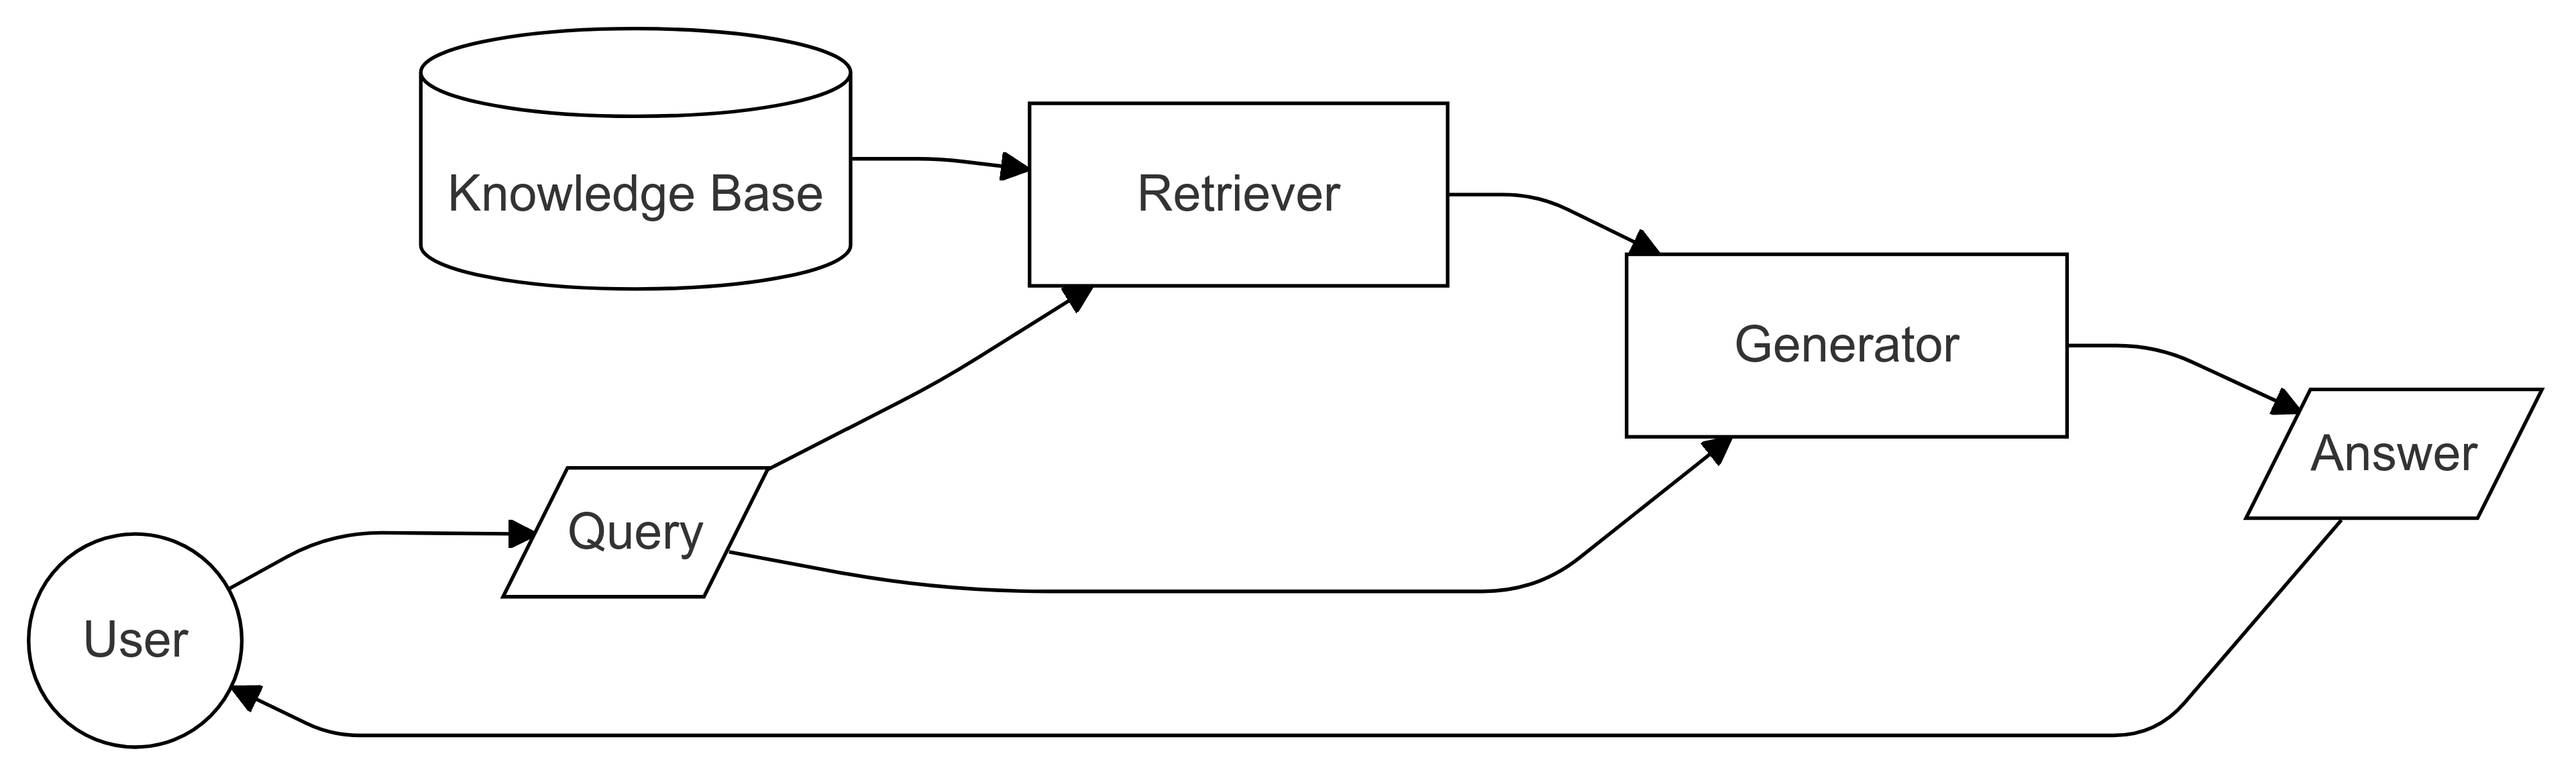
\includegraphics[width=0.8\textwidth]{figuras/rag-flow.png}
  \label{fig:rag-flow}
  \caption{Information flow in a RAG system}
\end{figure}

The generation process follows three fundamental steps:

\begin{enumerate}
  \item \textbf{Retrieval of relevant documents}: The system vectorizes the user's query and searches the knowledge base using semantic indices to find related documents.

  \item \textbf{Analysis and ranking of documents}: The relevance of retrieved documents is evaluated considering their semantic similarity with the query and the reliability of the sources.

  \item \textbf{Response generation}: The \gls{llm} integrates the retrieved knowledge with the context of the query to produce a coherent and precise response.
\end{enumerate}

\subsection{Applications and Advantages of RAG in Education}

\gls{rag} systems offer significant benefits for educational applications, especially in language teaching. The main advantages include:

\begin{itemize}
  \item \textbf{Precision and Reliability:} Greater precision in the provided information by combining structured knowledge with the flexibility of \gls{llm}s, reducing \gls{hallucinations} and incorrect responses by anchoring generation in reliable sources.

  \item \textbf{Traceability and Verifiability:} Ability to cite sources and relevant materials, providing verifiable references for educational content.

  \item \textbf{Adaptability and Updating:} These systems offer adaptability to different domains through knowledge base updates. This allows for dynamic content updating without the need to retrain the entire model. Additionally, it facilitates the personalization of educational content through the specific selection of relevant sources for each student.
\end{itemize}

\section{Reinforcement Learning}

\subsection{Theoretical Foundations of RL}

Reinforcement Learning provides an ideal mathematical framework for personalizing language learning. Based on \gls{mdp}, it allows modeling the learning process as a series of sequential decisions, where the system must select the most appropriate activities and content according to the student's level and progress \cite{williams2017educational}.

In our context, the state represents the student's current profile, including their language proficiency in different areas (comprehension, production, vocabulary, grammar), while actions correspond to the different available pedagogical interventions.

\subsection{Proximal Policy Optimization (PPO)}

PPO \cite{schulman2017proximal} is a \gls{rl} algorithm that stands out for its stability and efficiency in policy learning. In our language learning system, PPO is used to optimize activity selection and content adaptation.


\subsubsection{Mathematical Formulation}
The objective of PPO is to maximize the following objective function:

\begin{equation}
  L^{CLIP}(\theta) = \hat{\mathbb{E}}_t[\min(r_t(\theta)\hat{A}_t, \text{clip}(r_t(\theta), 1-\epsilon, 1+\epsilon)\hat{A}_t)]
\end{equation}

Where:

\begin{itemize}
  \item $r_t(\theta)$ is the probability ratio between the new and old policy
  \item $\hat{A}_t$ is the advantage estimation
  \item $\epsilon$ is the clipping parameter (typically 0.2)
\end{itemize}

\begin{algorithm}[H]
  \label{alg2}
  \SetAlgoLined
  \medskip
  \begin{enumerate}
    \item Inicializar los parámetros de la política $\theta$ y el valor función $\phi$
    \item Para cada iteración:
          \begin{enumerate}
            \item Recopilar conjunto de trayectorias $\mathcal{D}_k = \{\tau_i\}$ ejecutando la política $\pi_\theta$ en el entorno
            \item Calcular ventajas estimadas $\hat{A}_t$ usando función de valor actual $V_\phi$
            \item Para cada época de optimización:
                  \begin{enumerate}
                    \item Calcular ratio de probabilidad $r_t(\theta) = \frac{\pi_\theta(a_t|s_t)}{\pi_{\theta_{old}}(a_t|s_t)}$
                    \item Calcular pérdida recortada:
                          $$L^{CLIP}(\theta) = \hat{\mathbb{E}}_t[\min(r_t(\theta)\hat{A}_t, \text{clip}(r_t(\theta), 1-\epsilon, 1+\epsilon)\hat{A}_t)]$$
                    \item Actualizar $\theta$ minimizando $-L^{CLIP}(\theta)$ usando descenso de gradiente
                    \item Actualizar función de valor $\phi$ minimizando error cuadrático medio
                  \end{enumerate}
            \item Actualizar $\theta_{old} \leftarrow \theta$
          \end{enumerate}
    \item Devolver la política optimizada $\pi_\theta$
  \end{enumerate}
  \caption{Algoritmo \textit{Proximal Policy Optimization} (PPO)}
\end{algorithm}

\subsubsection{Application in the System}

In our educational context:

\begin{itemize}
  \item \textbf{State ($\mathcal{S}$):} Represents the student's current profile.
        \begin{equation}\label{eq:state}
          \mathcal{S} = \{\text{vocabulary\_level} = \text{B1}, \text{grammar\_level} = \text{A2}, \text{pronunciation\_level} = \text{B2}\}
        \end{equation}

  \item \textbf{Actions ($\mathcal{A}$):} Selection of activities and their parameters.
        \begin{equation}\label{eq:actions}
          \mathcal{A} = \{\text{grammar\_exercise\_A2}, \text{vocabulary\_practice\_B1}, \text{pronunciation\_dialogue\_B2}\}
        \end{equation}

  \item \textbf{Reward ($\mathcal{R}$):} Evaluates the success of each action. For example, if after a grammar exercise the student improves their accuracy from 60\% to 80\%, $\mathcal{R} = +20$

  \item \textbf{Policy ($\pi$):} Determines which action to take in each state. For example, if the student consistently shows errors in grammar, $\pi$ will select more grammar exercises
\end{itemize}

\subsubsection{Reward System}

The \gls{reward-function} is specifically designed for language learning, evaluating performance and providing feedback through multiple dimensions:

\begin{itemize}
  \item \textbf{Immediate rewards:} Include accuracy in responses and exercises, improvement in pronunciation and fluency, correct use of grammatical structures, and the acquisition and retention of vocabulary.

  \item \textbf{Long-term rewards:} Consider sustained progress in multiple linguistic dimensions, improvement in general communicative competence, and the retention and application of previous knowledge.

  \item \textbf{Dynamic adjustments:} Include automatic calibration of reward weights, adaptation to different learning styles and speeds, and balancing between different linguistic competencies.
\end{itemize}

\subsection{Evaluation of Learning Policies}

The evaluation of the \gls{policy} in language learning systems requires a multidimensional approach that considers both quantitative and qualitative aspects. \cite{williams2017educational} proposes an evaluation framework that examines:

\begin{itemize}
  \item \textbf{Progress in specific linguistic competencies:} Includes improvement in grammatical accuracy and use of structures, expansion of active and passive vocabulary, development of fluency and pronunciation, and advancement in listening and reading comprehension.

  \item \textbf{Effectiveness of personalization:} Encompasses adaptation to individual learning styles, response to specific error patterns, dynamic adjustment of difficulty level, and thematic content personalization.

  \item \textbf{Efficiency in learning time:} Considers the rate of acquisition of new concepts, reduction in skill mastery time, optimization of review intervals, and minimization of redundancy in exercises.

  \item \textbf{Student engagement and retention:} Evaluates levels of active participation, activity completion rates, persistence in the learning program, and satisfaction reported by the student.
\end{itemize}

The evaluation is performed using specific quantitative metrics:

\begin{equation}
  \text{Effectiveness} = \frac{\text{Objectives Achieved}}{\text{Time Invested}} \times \text{Difficulty Factor}
\end{equation}

\begin{equation}
  \text{Personalization Index} = \frac{\sum_{i=1}^{n} \text{Successful Adaptations}_i}{n} \times \text{Progress Rate}
\end{equation}

These metrics are complemented with continuous qualitative analysis and direct feedback from students to ensure a holistic evaluation of the \gls{policy}.


\section{Voice Processing Technologies}

Voice processing in language learning systems involves two fundamental processes: automatic speech recognition (\gls{stt}) and speech synthesis (\gls{tts}). These processes represent complementary transformations between the acoustic and linguistic domains.

\subsection{Automatic Speech Recognition (STT)}

The STT process transforms acoustic signals into text, involving multiple stages of processing and analysis. This process is based on principles of signal processing and probabilistic language models \cite{graves2013speech}.

\subsubsection{Acoustic Signal Processing}

\begin{itemize}
  \item \textbf{Acoustic Preprocessing:} The raw audio signal undergoes noise reduction techniques, amplitude normalization, and segmentation into frames. This process improves signal quality and prepares it for subsequent analysis.

  \item \textbf{Feature Extraction:} Spectral representations such as \gls{mfcc} coefficients are extracted, which capture the relevant acoustic features for speech recognition.

  \item \textbf{Feature Normalization:} The extracted features are normalized to reduce non-linguistic variations such as differences in volume or recording channel.
\end{itemize}

\subsubsection{Recognition Process}

\begin{itemize}
  \item \textbf{Acoustic Modeling:} The relationship between acoustic features and phonetic units of speech is analyzed, considering variations in pronunciation and phonetic context.

  \item \textbf{Language Modeling:} Knowledge about language structure is incorporated, including probabilities of word sequences and grammatical constraints.

  \item \textbf{Decoding:} Acoustic and linguistic information is combined to determine the most probable sequence of words, using search algorithms such as \gls{viterbi} or \gls{beam-search}.
\end{itemize}

\subsection{Speech Synthesis (TTS)}

Speech synthesis performs the inverse transformation, converting text into speech signals through a process that combines linguistic analysis and acoustic signal generation \cite{taylor2009text}.


\subsubsection{Linguistic Processing}

\begin{itemize}
  \item \textbf{Text Analysis:} The input text is processed to identify its linguistic structure, including tokenization, normalization, and syntactic analysis.

  \item \textbf{Grapheme-to-Phoneme Conversion:} Written text is transformed into its phonetic representation, considering pronunciation rules and language-specific exceptions.

  \item \textbf{Prosodic Analysis:} Patterns of intonation, duration, and emphasis are determined based on the syntactic and semantic structure of the text.
\end{itemize}

\subsubsection{Voice Generation}

\begin{itemize}
  \item \textbf{Prosodic Modeling:} Detailed patterns of pitch, duration, and energy are generated for each phoneme, considering the linguistic and emotional context.

  \item \textbf{Acoustic Feature Generation:} Intermediate spectral representations are produced that encode the desired acoustic properties of speech.

  \item \textbf{Waveform Synthesis:} The final audio signal is generated through synthesis techniques that can be concatenative, parametric, or based on neural models.
\end{itemize}

\subsection{Integration in Learning Systems}

The combination of STT and TTS in educational systems allows for creating complete cycles of oral interaction:

\begin{itemize}
  \item \textbf{Feedback Cycle:} The system can generate pronunciation examples (TTS), analyze the student's production (STT), and provide specific feedback.

  \item \textbf{Precision Analysis:} The comparison between the transcription of the student's speech and the target text allows evaluation of pronunciation precision and fluency.

  \item \textbf{Dynamic Adaptation:} The analysis results allow adjusting parameters such as speech speed, content complexity, and pronunciation acceptance threshold.
\end{itemize}